\section{Theorie}
Bei Röntgenstrahlung handelt es sich um durch das Abbremsen von geladenen Teilchen erzeugte elektromagnetische Strahlung mit Energien über $\SI{100}{\electronvolt}$. Elektromagnetische Strahlung lässt sich aufgrund des Superpositionsprinzip als Linearkombination zweier linear polarisierter Wellen beschreiben, die senkrecht zueinander stehen.

\subsection{Röntgenstrahlung an einer Grenzfläche}
Beim Einfall auf eine ebene Grenzfläche mit Brechungsindex $n_2$ bietet es sich an, die beiden linear polarisierten Wellen so zu wählen, dass die eine senkrecht und die andere parallel zur Flächennormalen polarisiert ist. Diese Situation ist in \autoref{fig:fresnel} dargestellt.

\begin{figure}[H]
  \centering
  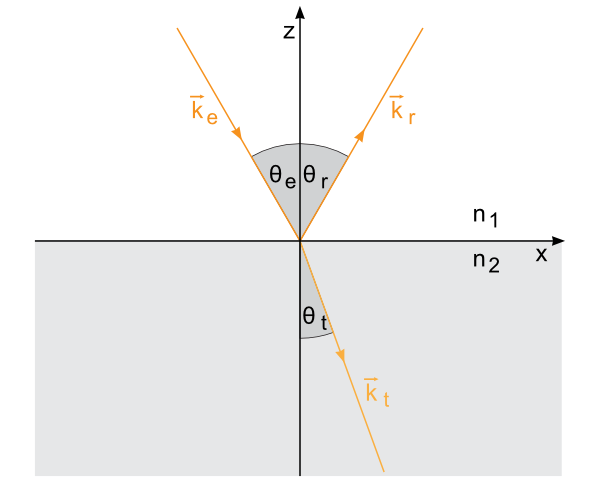
\includegraphics{fresnel.png}
  \caption{Eindimensionale Skizze zur Reflexion und Transmission von elektromagnetischer Strahlung an einer Grenzschicht \cite{fresnel}.}
  \label{fig:fresnel}
\end{figure}

In der Abbildung beschreiben $\vec{k}_\mathrm{e,r,t}$ den Wellenvektor der einfallenden (e), reflektierten (r) und transmittierten (t) Welle und $\theta_\mathrm{e,r,t}$ den jeweiligen Winkel zur Ebene.
Aufgrund des Snellius-Brechungsgesetz $n_1 \cos {\theta_\mathrm{e}} = n_2 \cos (\theta_\mathrm{a}) $ mit dem Ausfallswinkel $\theta_\mathrm{a}$ gilt $\theta_\mathrm{e} = \theta_\mathrm{r} \equiv \alpha$ und im weiteren Verlauf wird $\theta_\mathrm{t} \equiv \beta$ benutzt. Zur quantitativen Beschreibung der Transmission und Reflexion können die Fresnel-Gleichungen
\begin{align}
  \left( \frac{E_{0t}}{E_{0e}} \right)_{s}&=t_{s}=\frac{2 n _{1}\cos \alpha }{n_{1}\cos \alpha +\frac{\mu _{r1}}{\mu _{r2}}n_{2}\cos \beta }\\
  \left( \frac{E_{0r}}{E_{0e}} \right)_{s}&=r_{s}=\frac{n_{1}\cos \alpha -\frac{\mu _{r1}}{\mu _{r2}}n_{2}\cos \beta }{n_{1}\cos \alpha +\frac{\mu _{r1}}{\mu _{r2}}n_{2}\cos \beta } \\
  \left( \frac{E_{0t}}{E_{0e}} \right)_{p}&=t_{p}=\frac{2n_{1}\cos \alpha }{n_{2}\frac{\mu _{r1}}{\mu _{r2}}\cos \alpha +n_{1}\cos \beta }\\
  \left( \frac{E_{0r}}{E_{0e}} \right)_{p}&=r_{p}=\frac{n_{2}\frac{\mu _{r1}}{\mu _{r2}}\cos \alpha -n_{1}\cos \beta }{n_{2}\frac{\mu _{r1}}{\mu _{r2}}\cos \alpha +n_{1}\cos \beta }
  \label{fresnel}
\end{align}
genutzt werden, wobei die Indices $p$ und $s$ den parrallel und senkrecht polarisierten Anteil beschreiben. $E_0$ ist die jeweilige Amplitude des elektrischen Feldes und die $\mu_{ri}$ sind die magnetische Permeabilität der beiden Medien. Für nicht magnetische Materialen gilt $\frac{\mu_{r1}}{\mu_{r2}} \approx 1$ und ist das erste Medium das Vakuum gilt $n_1 = 1$. Weiterhin sind die Reflexionskoeffizienten für den senkrecht und parallel polarisierten Anteil näherungsweise gleich.
